\documentclass{standalone}

\usepackage[utf8]{inputenc}
\usepackage{amsfonts}
\usepackage{amssymb,amsmath}
\usepackage{tikz}
\usetikzlibrary{shapes,decorations.pathreplacing}

\begin{document}

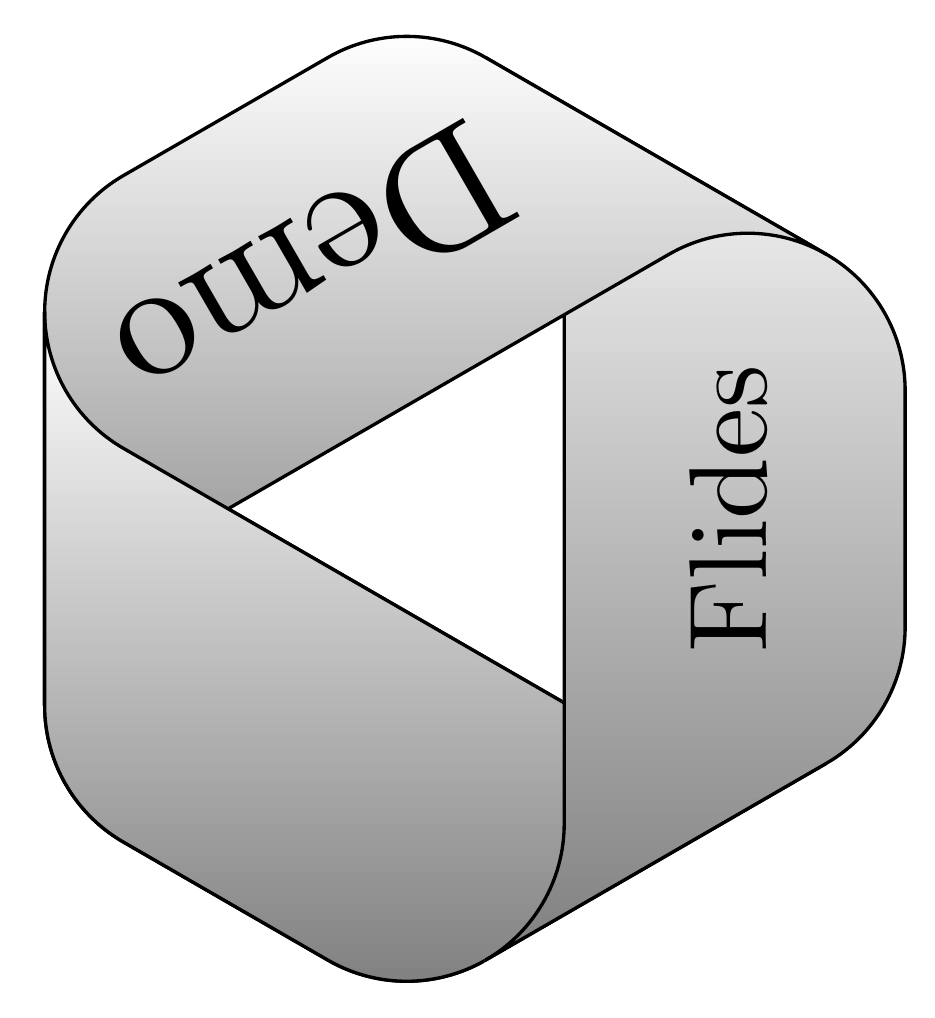
\begin{tikzpicture} [rotate=180]
\newcommand{\strip}[1]{%
\shadedraw[very thick,top color=white,bottom color=gray,rotate=#1]
 (0:2.8453) ++ (-30:1.5359) arc (60:0:2)
 -- ++  (90:5) arc (0:60:2) -- ++ (150:3) arc (60:120:2) 
 -- ++ (210:5) arc (120:60:2) -- cycle;}

%: \MoebiusStrip{<text1>}{<text2>}{<text3>}
\newcommand{\MoebiusStrip}[3]{%
\begin{scope} [transform shape]
    \strip{0}
    \strip{120}
    \strip{-120}
    \draw (-60:3.5) node[scale=6,rotate=30] {#1};
    \draw (180:3.5) node[scale=4,rotate=-90]{#3};
    % redraw the first strip after clipping
    \clip (-1.4,2.4)--(-.3,6.1)--(1.3,6.1)--(5.3,3.7)--(5.3,-2.7)--cycle;
    \strip{0}
    \draw (60:3.5) node [gray,xscale=-4,yscale=4,rotate=30]{#2};
\end{scope}}

\MoebiusStrip{Demo}{}{Flides}
\end{tikzpicture}

\end{document}